\chapter{Diseño del experimento}
En este capítulo se analizan los resultados que se obtuvieron al haber implementado el modelo, y se divide en tres partes.
En la primera de ellas se cuenta cómo es que se decidió implementar el modelo, así como también cuales de sus variables se dejaron fijas (serían constantes en esta implementación) y cuáles es posible variar desde la interfaz de usuario.

En la segunda parte se diseñaron ciertas pruebas con el fin de poner en evidencia características particulares del modelo, específicamente su correcto comportamiento físico.

Y en la última parte se hicieron dos tipos de pruebas para medir el desempeño del programa, variando la forma de ejecución y utilizando diferentes ambientes de ejecución.

\section{Definición del sistema}
En esta primera parte presento el experimento y explico qué parámetros fijé y cuáles pueden ser cambiados por el usuario.

\subsection{Características del modelo}
Tal como se explicó en la Seccion \ref{descripcion:experimento}, se modela un hexaedro regular, donde cinco de sus seis caras son rígidas y la cara superior o tapa es flexible: además, asumo que este hexaedro está relleno de gas.
En este sentido, el hexaedro completo o caja es el cuerpo neumático.
Mientras que la cara superior o tela es el cuerpo flexible.
Se le deja caer una esfera rígida, o pelota.
Un ejemplo del programa terminado se muestra en la Figura~\ref{programa:portada}.
\begin{figure}
 \centering
 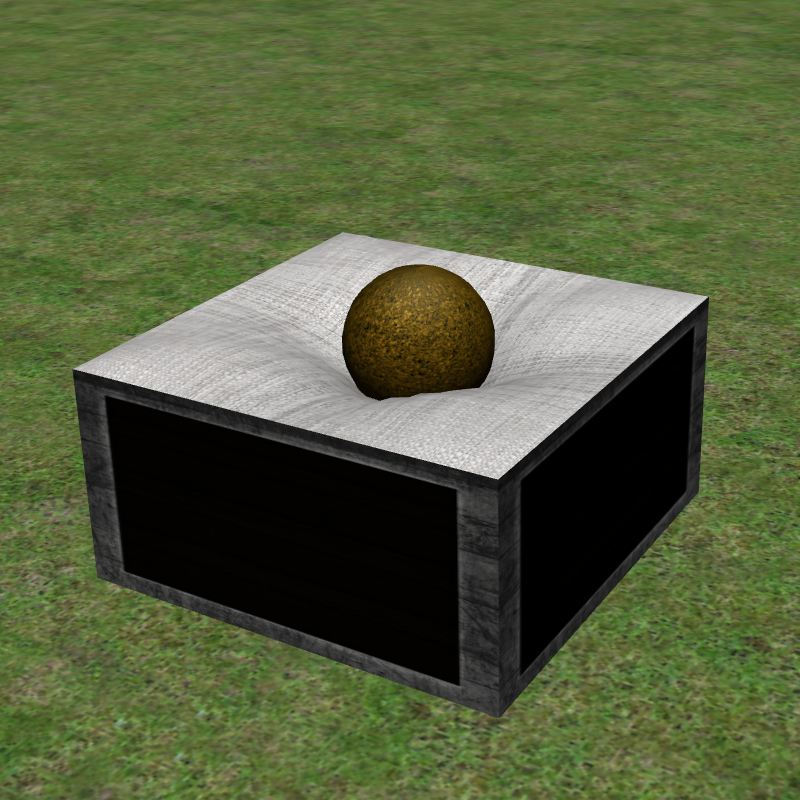
\includegraphics[width=0.85\textwidth]{Img/04/modeloPortada}
 \caption[Ejemplo del programa en ejecución]{Una imagen del programa que implementa el modelo.}
 \label{programa:portada}
\end{figure}

\subsubsection{Constantes del experimento}
En una situación como la antes descrita hay muchísimas variables del modelo, sin embargo al momento de hacer la implementación en código decidí dejar fijas algunas de ellas, es decir que la única manera de cambiarlas es modificando en el código fuente y recompilando el programa por completo.
Aquí está la lista de estas variables y su significado.

Las variables que se decidieron dejar fijas, y que por ende se convierten en constantes en el experimento son las siguientes:

\begin{itemize}
 \item El número de partículas por lado de la tela.
 \item Dimensiones (alto, ancho y largo) de la caja.
 \item La masa total de la tela. Y por lo tanto, la masa de cada partícula es ésta cantidad dividida entre el número total de partículas.
 \item El radio y la posición de la pelota.
 \item El tamaño del paso en el tiempo $\Delta t$ que se usa para los métods numéricos de integración.
\end{itemize}

Los valores de estas constantes con las que se hizo este experimento están en la tabla~\ref{valores:constantes}.
\begin{table}
\ra{1.2}
\begin{center}
\begin{tabular} {@{}lrp{10cm}@{}}
\toprule
Constante & Valor & Comentario\\ 
\midrule
 Número de partículas & 22 & Para que se vea mejor el modelo, se elige un número par\\
 Dimensiones caja & $0.75 \times 1.5 \times 1.5$ & Se forma una caja de tapas cuadradas \\
 Masa tela & 10 & La masa de cada particula es entonces $\frac{10}{22^{2}}$ \\
 Radio pelota & 0.25 &  \\
 Posición pelota & $(0, 1.5, 0)$& Como el cuerpo neumatico esta centrado en el origen. La pelota esta justo arriba de él en el centro\\
 $\Delta t$ & 0.0025 & Determinado experimentalmente \\
\bottomrule
\end{tabular}
\caption[Tabla con los valores de las constantes durante el experimento]{Valor de las constantes del experimento}
\label{valores:constantes}
\end{center}
\end{table}

\subsubsection{Variables físicas del experimento}
La variables físicas del experimento pueden ser modificadas en tiempo de ejecución por medio del menú que muestra en la Figura~\ref{programa:menu}.

\begin{figure}
 \centering
 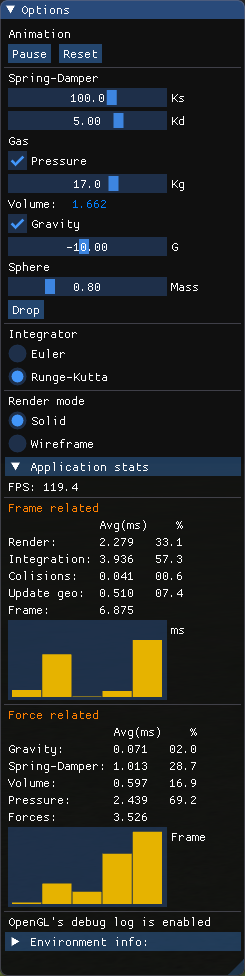
\includegraphics[width=0.5\textwidth]{Img/04/menu}
 \caption[Menú de usuario del programa]{Menú de usuario.}
 \label{programa:menu}
\end{figure}

Para la pelota o esfera (\emph{\textenglish{Sphere}}) que se refiere al cuerpo rígido.
la única variable que se puede modificar es su masa.

Los parámetros del cuerpo flexible que es posible modificar se dividen en tres subcategorias una por cada fuerza que se acumula.

La categoria del \emph{Gas}, al que se puede prender o apagar por medio del checkbox \emph{\textenglish{Pressure}}. 
Además, se puede modular su magnitud variando el valor de la constante $k_{g}$, por medio del control.

La de la \emph{\textenglish{Gravity}}, que al igual que la anterior se puede prender o apagar con el control  y también se puede modular variando el valor de la constante $g$.

Por últim subcategoria es la debida al resorte amortiguador (\emph{\textenglish{Spring-Damper}}.)
Esta fuerza no se puede apagar, pero se puede variar modificando dos parámetros $k_{s}$, que, como ya se dijo, controla la rigidez del resorte y $k_{d}$ que controla el amortiguamiento o pérdida de energía debida al resorte.

Aunque no es propiamnete una opción de la física. El menú tambien permite elegir que método numérico usar para integrar.
Las opciones disponibles son: \emph{Euler} y \emph{Runge-Kutta}.

Los valores de default de estas variables (el valor que tiene al iniciar la ejecución) son los que muestra la Tabla~\ref{valores:variables}.

\begin{table}
\ra{1.2}
\begin{center}
%\begin{tabular} {|c|c|p{10cm}|}
\begin{tabular} {@{}llp{10cm}@{}}
\toprule
Parametro & Valor & Comentario\\
\midrule
 Masa & 0.08 & Masa del cuerpo rígido \\
 Integrador & Euler & Método Numérico con el que se integra. \\
 Gas & Activado & El programa empieza con la fuerza del gas prendida \\
 $k_g$ & 17 & Constante de presión del gas \\
 Gravedad & Activada & La gravedad está activada \\
 $g$ & -10.0 & La gravedad es negativa (jala hacia abajo) \\
 $k_s$ & 100 & La fuerza de los resortes \\
 $k_d$ & 5 & El valor de damping \\
\bottomrule
\end{tabular}
\end{center}
\caption[Tabla con los valores de defecto de los parámetros]{Valor inicial de los parámetros del experimento}
\label{valores:variables}
\end{table}

\subsubsection{Opciones de control y visualización}
Hay otras opciones que se pueden modificar por medio del menú, que se refieren más a como controlamos la animación y a como se ve el modelo que a la física.

Dentro de las del flujo de la animación, sólo hay dos controles, el de \emph{\textenglish{Pause/Play}}, que puede detener (reanudar) la animación física (se sigue pudiendo mover la cámara).
Y el botón de \emph{\textenglish{Reset}}, que devuelve a todos los objetos a su posición original.

El botón de \emph{\textenglish{Drop}}, hace que la esfera se deje caer.

Dentro de la categoría de \emph{\textenglish{Render}}, se encuentran las siguientes opciones:

La primera opción \emph{\textenglish{solid}}, usa el modelo de iluminación de Phong (los materiales se obtiene de texturas) para dibujar todos los objetos en la escena.

Y la segunda opción \emph{\textenglish{wireframe}}. 
Que solo cambia la manera de dibujar el cuerpo neumático.
Dibuja con lineas azules las orillas de la caja y dibuja en una escala de color entre amarillo y rojo, los resortes (como lineas) y las particulas (como puntos) que forman el cuepor flexible.
El color asignado depende de la magnitud de la fuerza que actua sobre ellos.

Finalmente, además del menú de usuario, hay opciones que solo se pueden modificar por medio del \textenglish{mouse} y del teclado.

\begin{itemize}
 \item Arrastar el mouse con el botón izquierdo presionado, permite modificar el ángulo de la camara. Se usa el modelo de \emph{\textenglish{trackball camera}}.
 \item La rueda del mouse, cambia el \emph{\textenglish{zoom}} de la cámara.
 \item Presionar la tecla `\emph{s}' en el teclado toma un \emph{\textenglish{screenshot}}. Las imágenes son guardadas en el folder \mintinline{cpp}{Screenshoots} (Que debe ser creado por el usuario) en el mismo folder donde esta el ejecutable.
 \item Presionar \emph{Escape} en el teclado termina la ejecución del programa.
 \item Presionar la tecla `\emph{m}' muesta/oculta el menú de usuario.
 \item Presionar \emph{F11} cambia entre el modo de pantalla completa y de ventana.
 \item La tecla `\emph{p}' es un atajo para el boton de \emph{\textenglish{Play/Pause}} de la animación.
 \item La tecla `\emph{r}' es un atajo para el boton de \emph{\textenglish{Reset}} de la animación.
\end{itemize}

\subsection{Características del entorno de pruebas}

\subsubsection{Software}

El programa fue desarollado en lenguaje C++ y los shaders que sirven para hacer el render fueron escritos en GLSL.

Para poder compilar el código fuente de este programa es necesario tener un entorno de programación que contemple lo siguiente:

\begin{itemize}
 \item Un compilador de C++.
 \item La biblioteca OpenGL
 \item La biblioteca glfw
 \item La biblioteca Dear Imgui.
 \item La biblioteca GLM
 \item La biblioteca GLEW
 \item La biblioteca GLM
 \item La biblioteca FreeImage
 \item La biblioteca Assimp
\end{itemize}

Todas éstos requerimeintos son software libre (Mas detalles de esto en el Apéndice).
Aunque este trabajo fue desarollado en su totalidad en un sistema operativo GNU/Linux, todos los requerimeintos tienen la enorme ventaja de estar disponibles en cualquier plataforma.
Si las bibliotecas están correctamente instaladas, el programa y debe compilar y funcionar bajo cualquier sistema operativo.

\subsection{Hardware}
La mayoría de las pruebas fueron hechas en una laptop personal MSI GF65, con las siguientes características.

\begin{itemize}
\label{maquina:trabajo} 
 \item Procesador: Intel Core i7-9750H CPU @ 2.60GHz $\times$ 12.
 \item Memoria: 32GB DDR2.
 \item Tarjeta de Video: Nvidia GeForce GTX 1660 Ti Mobile\footnote{Aunque la laptop tiene la tarjeta de video descrita, el programa es tan simple que de hecho puede ejecutarse en la tarjeta de video integrada del procesador Intel sin problemas (Ver Figura~\ref{programa:menu})}.
 \item Sistema Operativo: Ubuntu 20.04 64bits.
\end{itemize}

Esto no quiere decir que este sea el hardware mínimo, sólo que la \emph{mayoría} de las pruebas se realiaron en este hardware.
Sin embargo, se ha ejecutado con éxito en equipos bastante accesibles. 
Éste trabajo es de hecho una reedición, el trabajo original se desarollo usando una laptop convencional en el año 2008.
Actualmente, éste programa debe poder ejecutarse en cualquier computadora personal, de escritorio o equipo movil sin problemas de capacidad del \emph{\textenglish{hardware}}.
Hoy en día la única limitante (de existir) podría acaso ser el \emph{\textenglish{software}}.

\section{Características físicas del modelo}
Para poner en a prueba la fidelidad del modelo, se hicieron las siguientes pruebas.
La mayoría para probar la sensibilidad del programa ante la variacion de sus parámetros físicos.

\subsection{Probando la gravedad}
La gravedad es la única fuerza que actúa tanto en el cuerpo flexible como en en el cuerpo rígido. Para entender mejor cómo afecta se sugieren las siguientes pruebas.

Partiendo de los valores de \emph{\foreignlanguage{english}{default}}, se espera a que la tela se estabilice (Figura~\ref{fig:testGEstable}).
Ahora se \emph{aumenta} la gravedad a su valor más \emph{pequeño} (recordemos que hacer la gravedad más fuerte es hacerla más negativa), es decir, $g=-20$, se observa ahora como la gravedad es muy fuerte como para que la presión del gas infle la tela, por lo que queda colgando un poco.
Las partículas que forman el cuerpo flexible son muy pesadas (son jaladas con más fuerza hacia abajo).
Esta situación se muestra en la Figura~\ref{fig:testGAumenta}. 
Ahora se deja caer la pelota y se espera que se estabilice de nuevo el programa, (Figura~\ref{fig:testGCae}) la gravedad hace que la pelota y las partículas pesen más, sin embargo la fuerza del gas que no se ha tocado compensa de alguna manera y no deja que se hunda más la pelota.
Con la pelota estable sobre la tela, apagué la fuerza del gas.
Al apagar la fuerza que equilibraba la gravedad todo se va hacia abajo, por la gravedad, pero como además esta fuerza es grande, la rigidez del resorte es poca para evitar un efecto de súper elongación como el que se ve en la Figura~\ref{fig:testGNoPres}, donde la pelota es detenida por el piso.

\begin{figure}
 \centering
  \begin{subfigure}[b]{0.45\textwidth}
    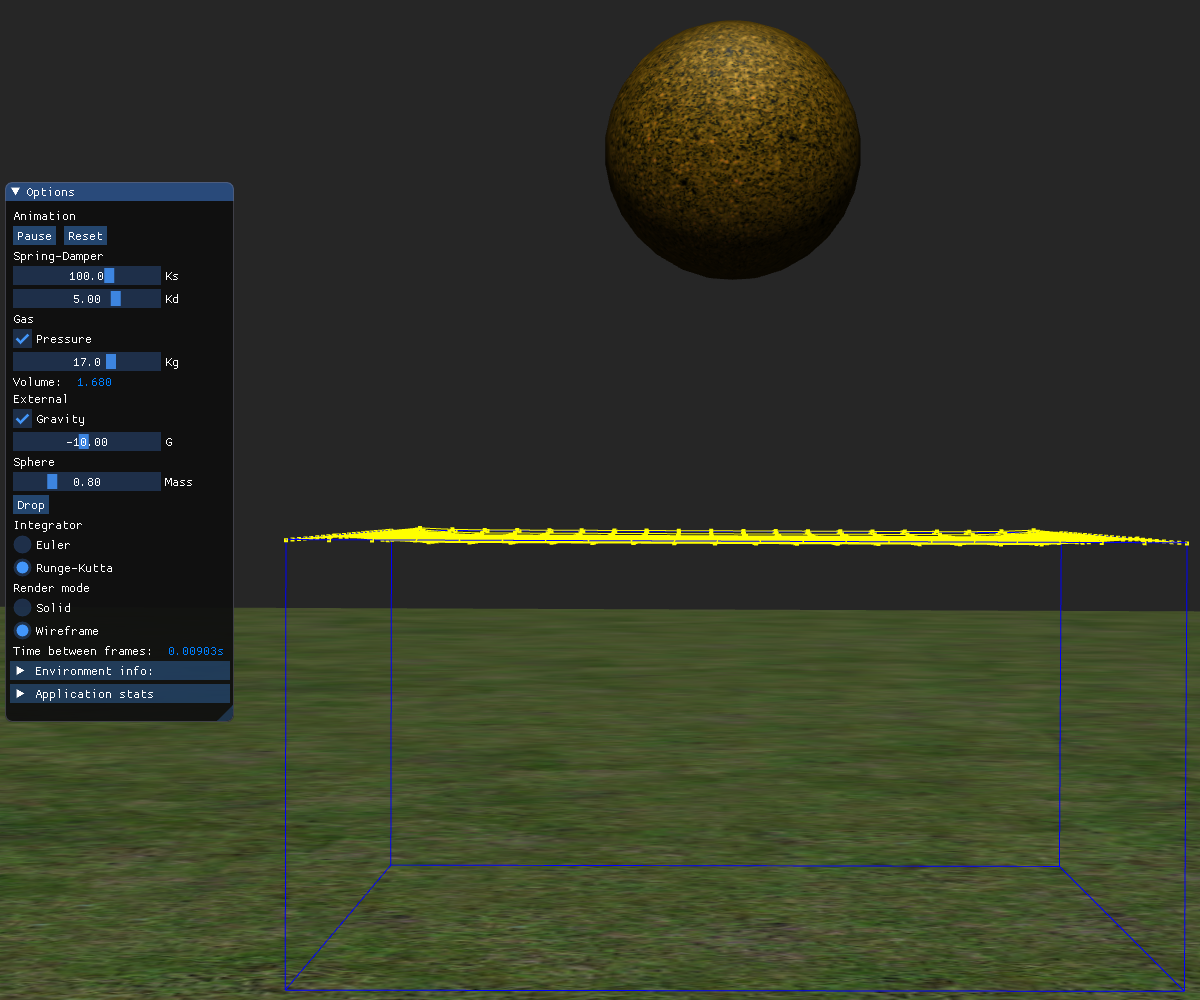
\includegraphics[width=\textwidth]{Img/04/gravity1}
    \caption{La tela se estabiliza con la gravedad y la presion.}
    \label{fig:testGEstable}
  \end{subfigure}
~
  \begin{subfigure}[b]{0.45\textwidth}
    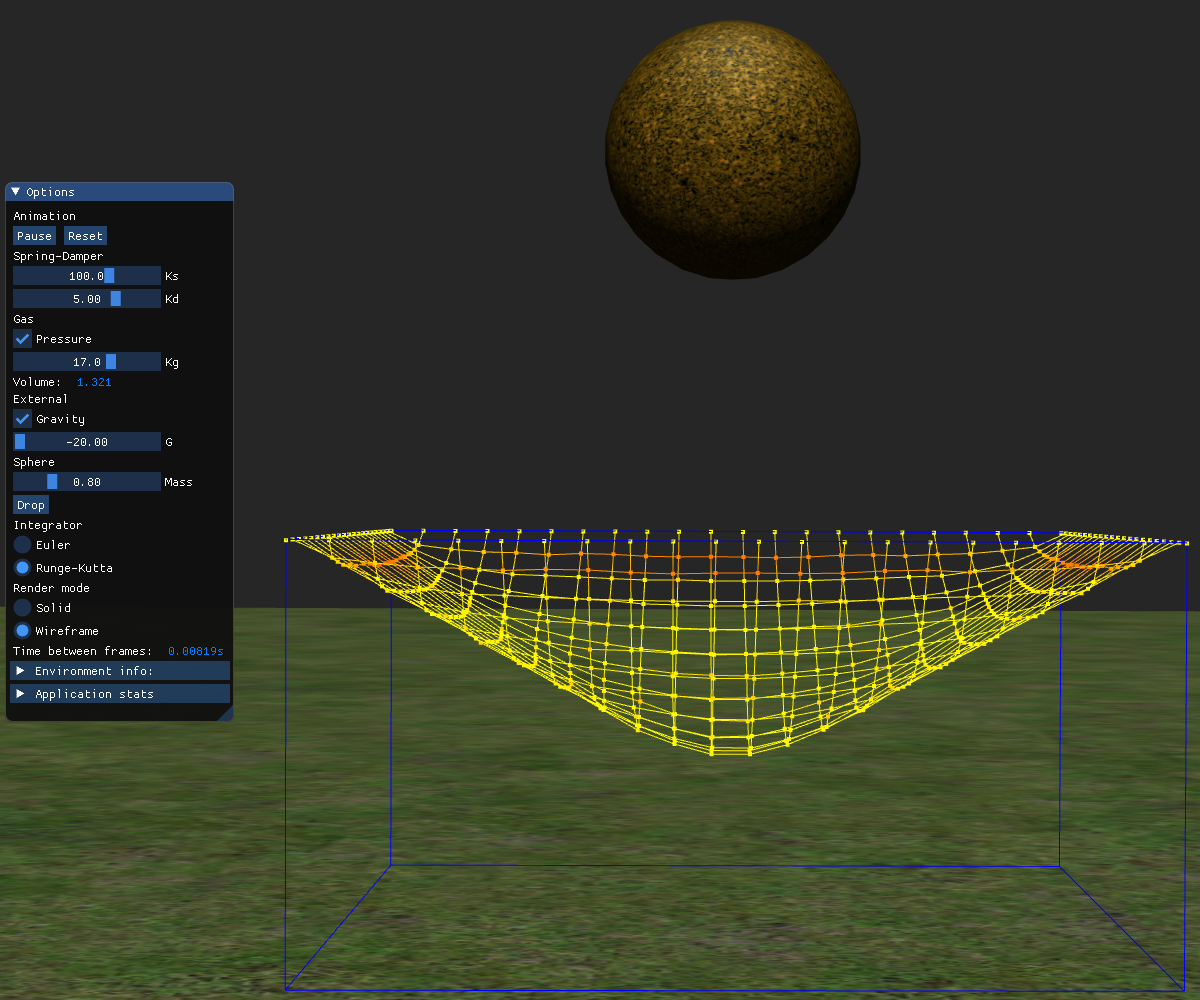
\includegraphics[width=\textwidth]{Img/04/gravity2}
    \caption{La gravedad aumenta a $g=-20$}
    \label{fig:testGAumenta}
  \end{subfigure}
\\
  \begin{subfigure}[b]{0.45\textwidth}
    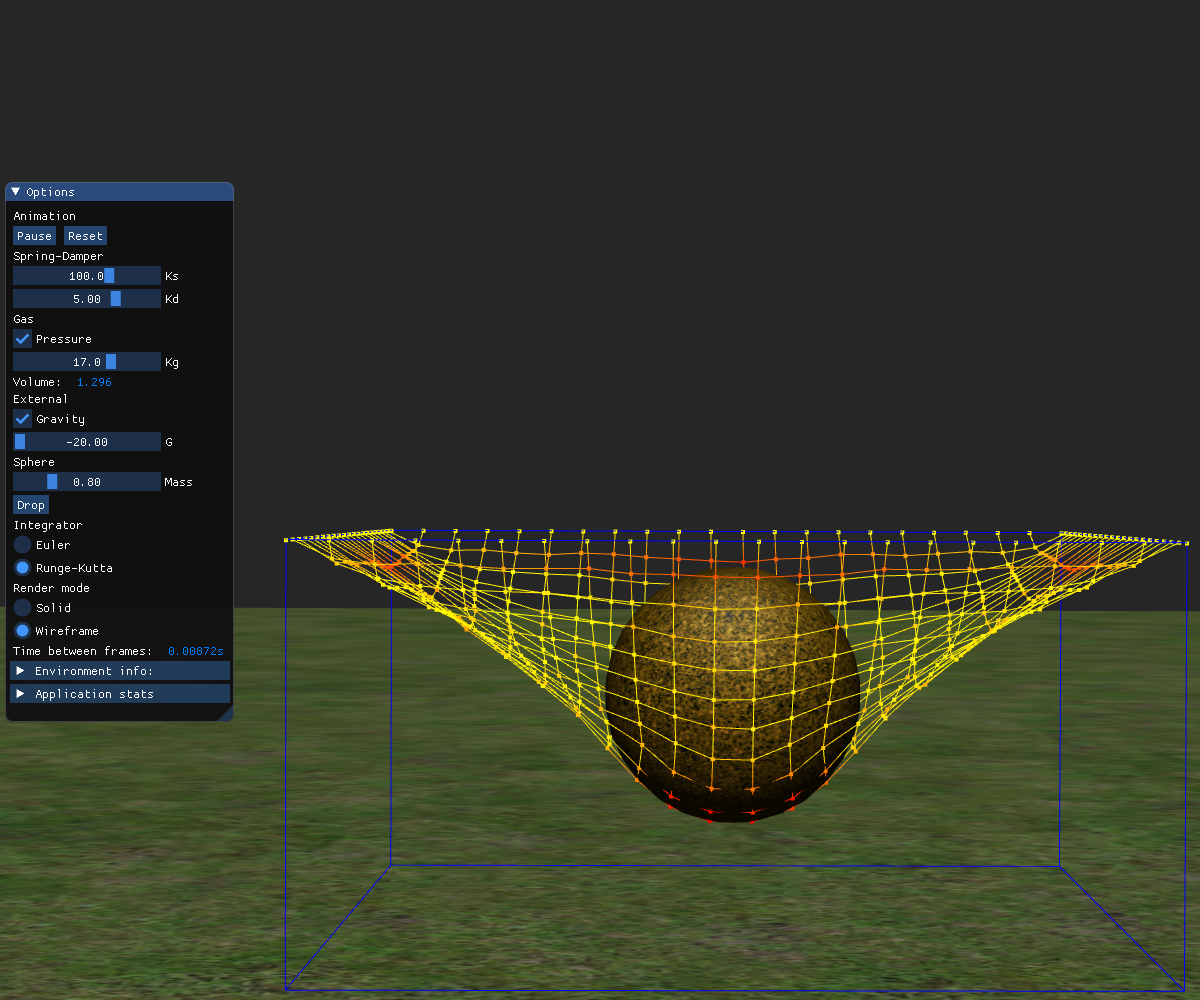
\includegraphics[width=\textwidth]{Img/04/gravity3}
    \caption{La pelota se deja caer.}
    \label{fig:testGCae}
  \end{subfigure}
~
  \begin{subfigure}[b]{0.45\textwidth}
    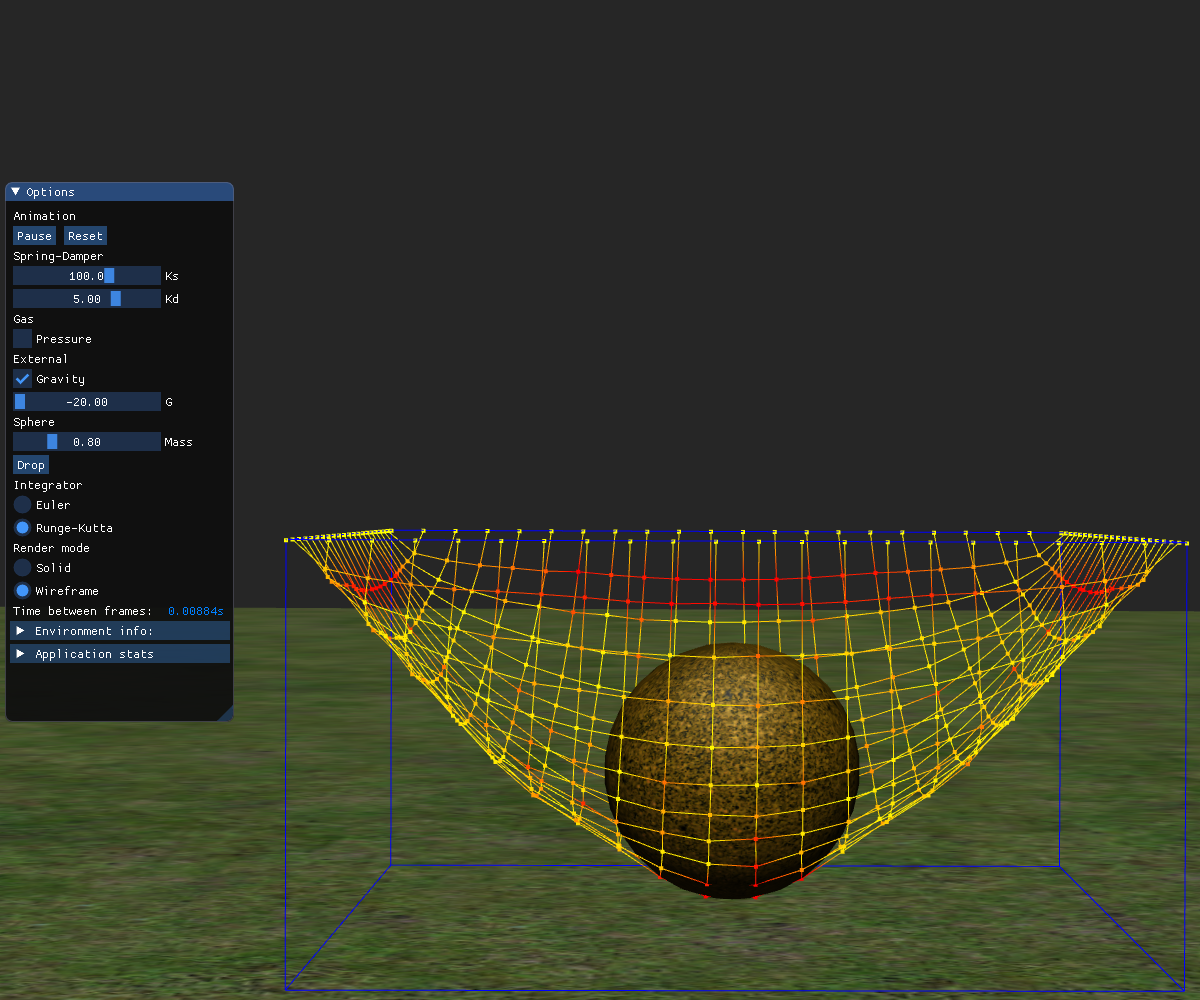
\includegraphics[width=\textwidth]{Img/04/gravity4}
    \caption{Se apaga la fuerza de presión}
    \label{fig:testGNoPres}
  \end{subfigure}
 \caption[Experimento: Fuerza de gravedad]{Probando la fuerza de gravedad} 
 \label{fig:testGravity}
\end{figure}

Reinicie la animación y vuelva a los valores de \emph{\foreignlanguage{english}{default}}.
De nuevo espere a que se estabilice la tela ahora disminuya la gravedad a su máximo valor posible, es decir una gravedad positiva: $g=1$.
Ahora verá que la tela se va más hacia arriba, como si se inflara más el cuerpo flexible, esto se debe a que ahora la gravedad no se opone a la presión del gas, sino mas bien le favorece, por lo que el cuerpo flexible, es jalado hacia arriba aún más, como se ve en la Figura~\ref{fig:testGpos1}.
Ahora deje caer la pelota, como la gravedad es positiva y pequeña (su valor absoluto en una décima parte del valor normal) la pelota \emph{sube lentamente}, y se aleja del cuerpo flexible (Figura~\ref{fig:testGpos2}).
La constante de gravedad influencía la velocidad de caída de los cuerpos.

\begin{figure}
 \centering
  \begin{subfigure}[b]{0.45\textwidth}
    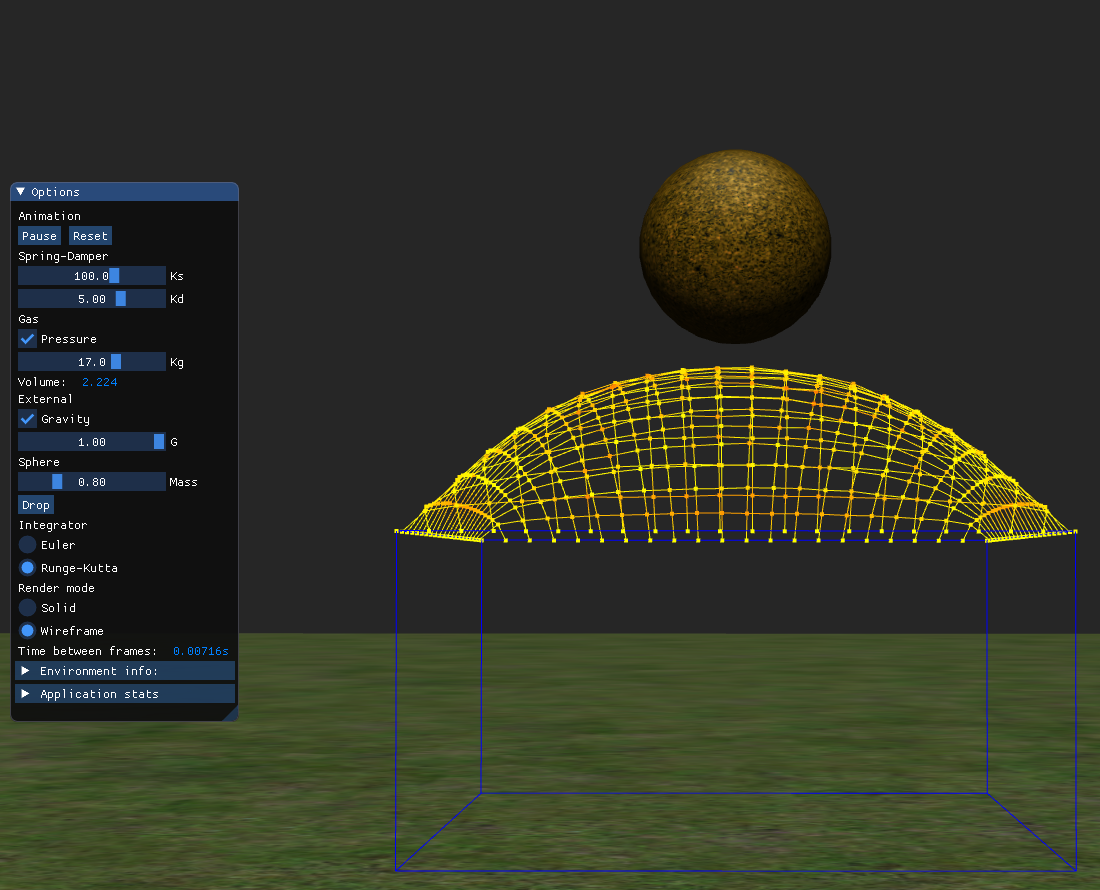
\includegraphics[width=\textwidth]{Img/04/positiveGravity1}
    \caption{La presion y la gravedad jalan la tela hacia arriba.}
    \label{fig:testGpos1}
  \end{subfigure}
~
  \begin{subfigure}[b]{0.45\textwidth}
    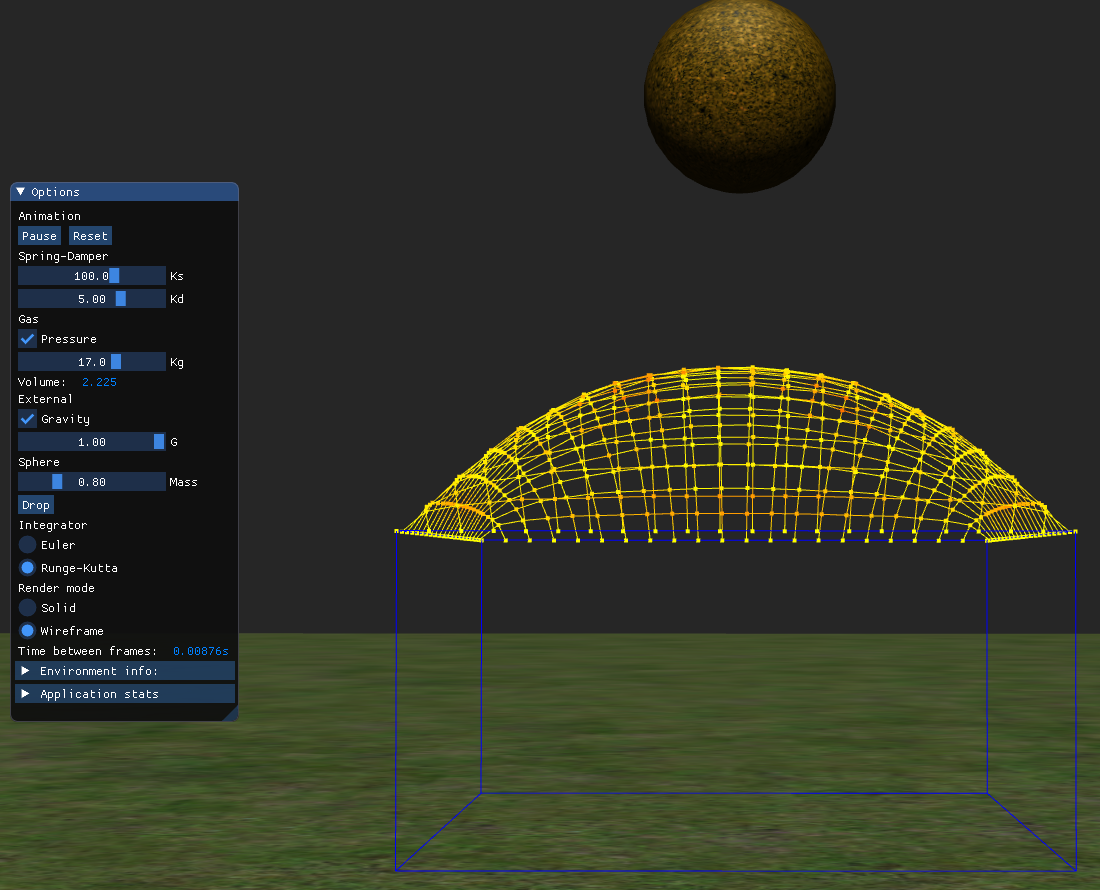
\includegraphics[width=\textwidth]{Img/04/positiveGravity2}
    \caption{La pelota también es jalada hacia arriba}
    \label{fig:testGpos2}
  \end{subfigure}
 \caption[Experimento: $g > 0$]{La fuerza de gravedad cambia de signo} 
 \label{fig:positiveGravity}
\end{figure}

Por último vamos a reiniciar la animación y partiendo de los valores de \emph{\foreignlanguage{english}{default}} de los parámetros, se apaga la gravedad. 
Este comportamiento equivale a hacer $g=0$ con la diferencia de que se hacen menos cálculos, ahora vemos cómo de nuevo la tela se mueve hacia arriba, cómo la gravedad se oponía a la fuerza del gas y ya no está, el gas empuja la tela aún más hacia arriba.
Si en esta situación se deja caer la pelota no pasará nada, debido a que la caída de la pelota \emph{depende de la gravedad}, y al no haber, simplemente no hay caída.

Si primero se deja caer la pelota sobre la tela, y una vez que esta se estabiliza se apaga la gravedad, la pelota es empujada afuera del cuerpo flexible por un impulso. Ver la Figura~\ref{fig:noGravity}.

\begin{figure}
 \centering
  \begin{subfigure}[b]{0.3\textwidth}
    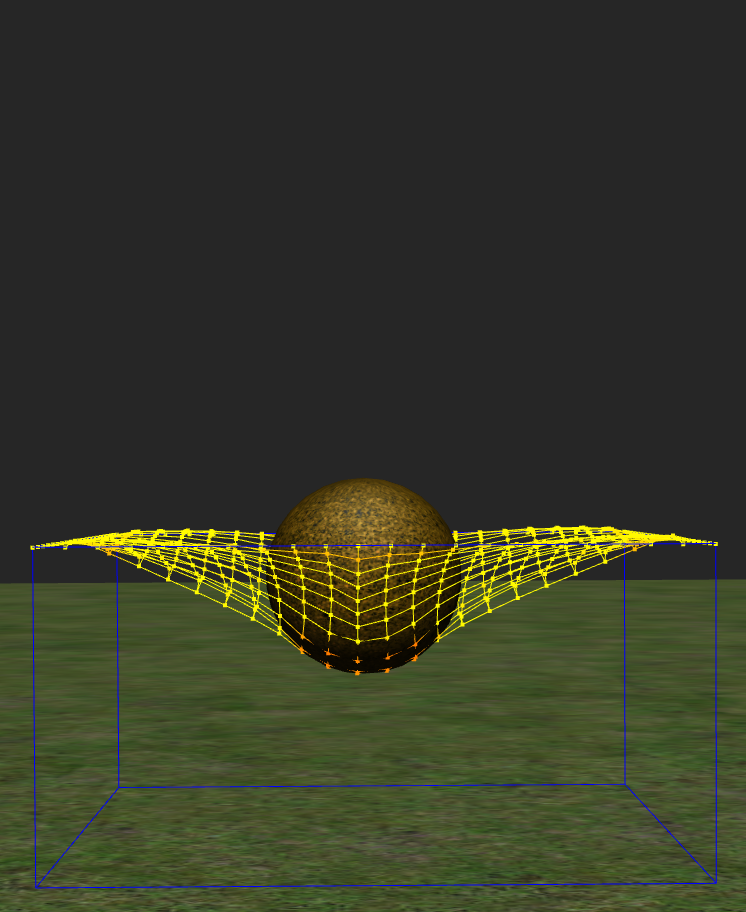
\includegraphics[width=\textwidth]{Img/04/gravityOff1}
  \end{subfigure}
~
  \begin{subfigure}[b]{0.3\textwidth}
    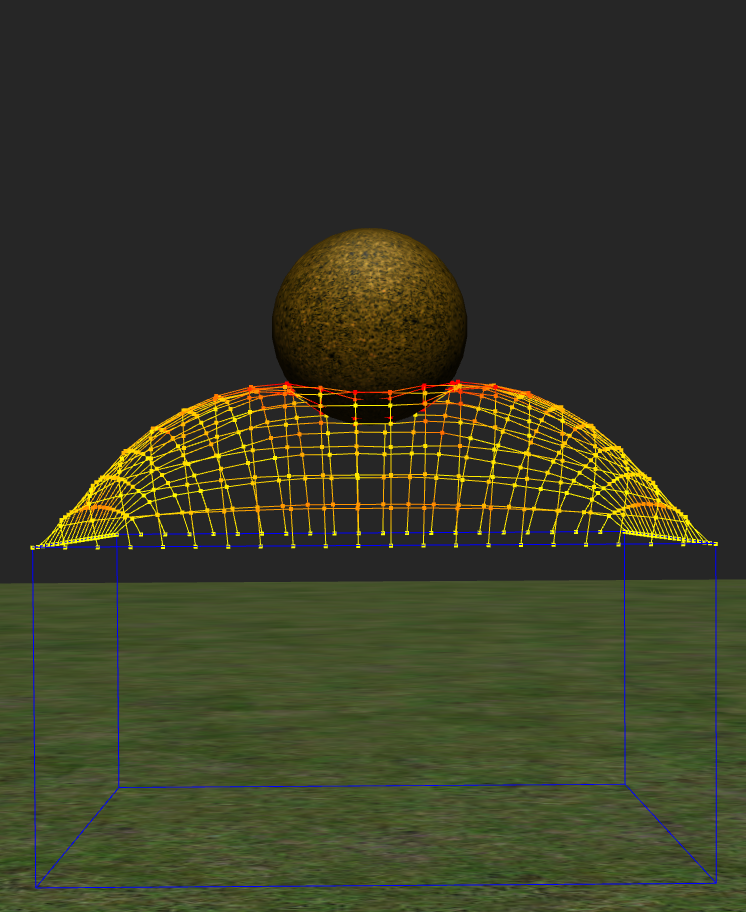
\includegraphics[width=\textwidth]{Img/04/gravityOff2}
  \end{subfigure}
~
  \begin{subfigure}[b]{0.3\textwidth}
    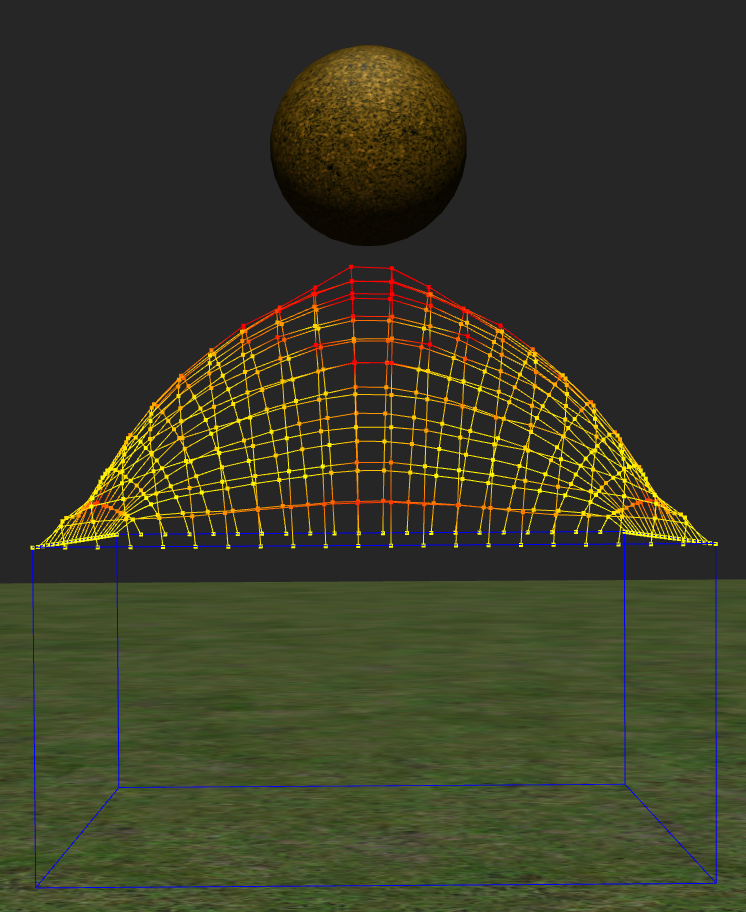
\includegraphics[width=\textwidth]{Img/04/gravityOff3}
  \end{subfigure}
 \caption[Experimento: Apagar la fuerza de gravedad]{La fuerza de gravedad es apagada después de que la pelota descansa sobre la tela.} 
 \label{fig:noGravity}
\end{figure}

\subsection{Probando la fuerza del gas}
Ahora se harán pruebas sobre la fuerza del gas. La fuerza del gas, por el diseño de nuestro experimento, se opone a la fuerza de gravedad, y actúa sólo sobre el cuerpo flexible, sin embargo tiene cierto efecto sobre la velocidad de las partículas del cuerpo flexible, que a su vez tienen cierto efecto sobre el cuerpo \emph{rígido} al momento de la colisión.

Inicie el programa con los valores de \emph{\foreignlanguage{english}{default}}, ahora apague la fuerza del gas y espere a que se estabilice el modelo, como se ve el la figura~\ref{pres:test1}.
Como no hay fuerza del gas, la tela o cuerpo flexible cuelga agarrada de las orillas de la caja.
Ahora deje caer la pelota sobre el cuerpo flexible y espere a que se estabilice la animación, justo como se ve en la figura~\ref{pres:test2}. 
Prenda la fuerza del gas y observe como la pelota es lanzada hacia arriba súbitamente como se ve en la figura~\ref{pres:test3}.

\begin{figure}
 \centering
 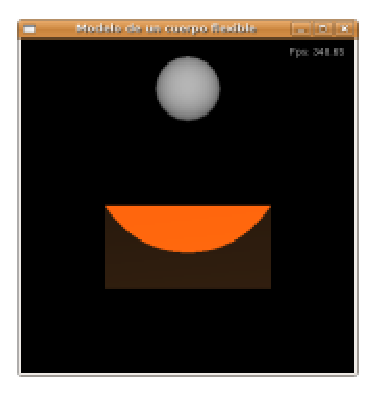
\includegraphics[]{Img/modPres1}
 \caption[Ejecución con la fuerza del gas apagada]{Fuerza del gas apagada.}
 \label{pres:test1}
\end{figure}

\begin{figure}
 \centering
 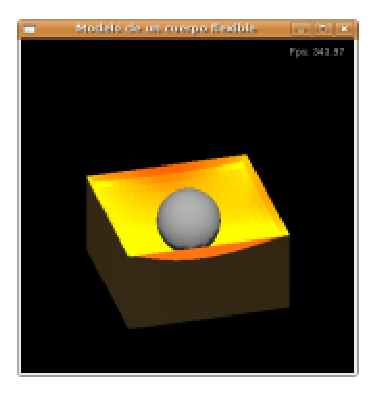
\includegraphics[]{Img/modPres2}
 \caption[Ejecución con la esfera cayendo en ausencia de fuerza del gas]{La pelota cae mientras está apagado el gas.}
 \label{pres:test2}
\end{figure}

\begin{figure}
 \centering
 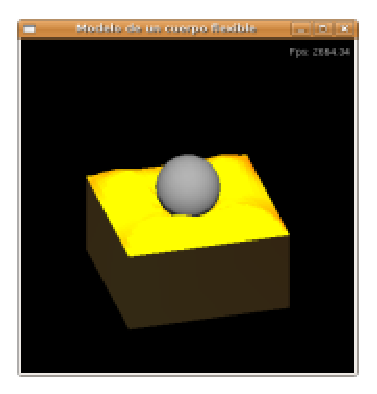
\includegraphics[]{Img/modPres3}
 \caption[Ejecución con la esfera lanzada por la fuerza del gas]{La pelota es lanzada por la fuerza del gas.}
 \label{pres:test3}
\end{figure}

Otra prueba es ver los efectos de la variación de la constante $k_g$.
Inicie la animación con los valores de \emph{\foreignlanguage{english}{default}} y haga la constante $k_g$ pequeña, por ejemplo $k_g =$ 350.0; verá cómo el gas no es lo suficientemente fuerte para inflar el cuerpo flexible.
Ahora aumente poco a poco la constante $k_g$ y observe cómo se infla cada vez más el cuerpo flexible.
En la figura~\ref{pres:test4} se ilustran estas situaciones para diferentes valores en aumento de la constante $k_g$.

\begin{figure}
 \centering
 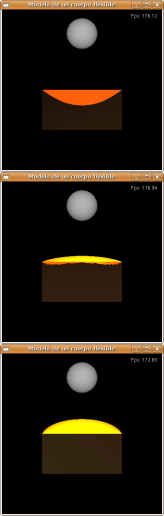
\includegraphics[]{Img/modPres4}
 \caption[Ejecución con diferentes valores de la constante de gas]{Variando la fuerza del gas: $k_g=$350.0 (arriba), $k_g=$730.0 (centro), $k_g=$970.0 (abajo)}
 \label{pres:test4}
\end{figure}

\subsection{Probando los resortes amortiguadores}
La siguientes pruebas sirven para mostrar cómo funcionan los resortes amortiguadores.
Primero vamos a hacer una prueba con la constante de \emph{\foreignlanguage{english}{damping}} $k_d$.
Como ya se dijo, el damping es una forma de perder energía del sistema y, por lo tanto, de eventualmente estabilizarse.
Iniciemos la animación con los valores de \emph{\foreignlanguage{english}{default}} y hagamos la constante $k_d=0$, es decir quitemos todo el \emph{\foreignlanguage{english}{damping}}.
Vemos que la tela empieza a oscilar rápidamente como consecuencia del gas.
Ahora quitemos también el gas y esperemos un momento; veremos como la tela oscila sin detenerse ni estabilizarse en ningún momento, es cierto que cada vez oscila menos, pero ciertamente tardará mucho en detenerse (o nunca se detendrá).

En la figura~\ref{res:test1}, podemos ver diferentes oscilaciones sin control por falta de un amortiguador.
Como ya se había dicho, el amortiguador agrega realismo (en la total ausencia de \emph{\foreignlanguage{english}{damping}}, el cuerpo flexible se ve poco real). La contra parte es que a mayor \emph{\foreignlanguage{english}{damping}}, también hay menos estabilidad numérica, por lo que el modelo es sumamente sensible al aumento en este parámetro.

Podemos ir aumentando el valor de $k_d$ poco a poco y ver cómo el modelo se vuelve inestable, podemos por ejemplo poner el máximo posible $k_d=$0.6 y reiniciar la animación, esperar a que se estabilice y apagar el gas, el modelo explota (ver figura~\ref{res:test4}).

Ahora analicemos la constante de rigidez $k_s$.
Esta constante hace a los resortes más poderosos, por lo que en general hace que las partículas que están unidas por ellos, se separen menos, es decir hace más estable el cuerpo flexible en general, además de prevenir el efecto de super elongación.

Iniciamos la animación con los valores de default y pongamos la constante del resorte $k_s$ a su máximo valor.
Ahora apaguemos el gas y vemos como la caída de la tela es menor, sin embargo al apagar y prender varias veces el gas también nos damos cuenta de que el cuerpo flexible parece oscilar más, como consecuencia de que los resortes en general jalan más fuerte, tanto hacia arriba como hacia abajo.

Ahora con la constante $k_s$ en el máximo y el gas prendido, vayamos poco a poco subiendo la presión del gas, aumentando $k_g$ hasta su máximo $k_g=$2000.0. 
Podemos ver cómo aun llegando al máximo de $k_g$, el cuerpo flexible se expande poco; esperemos a que se estabilice, como se ve en la figura~\ref{res:test5}. 
Ahora que tenemos el modelo estable y con ambas constantes $k_s$ y $k_g$ al máximo, poco a poco vayamos haciendo $k_s$ más pequeña y podremos apreciar como el cuerpo parece inflarse más (la resistencia de la membrana que lo mantiene unido es menor), como se ve en la figura~\ref{res:test6}, hasta llegar al momento donde explota ($k_s$ = 0.0).

\begin{figure}
 \centering
 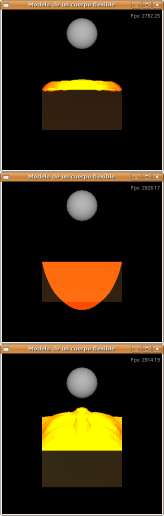
\includegraphics[]{Img/modRes1}
 \caption[Ejecución sin fuerza de amortiguamiento]{Oscilación sin control: $k_d$=0.0}
 \label{res:test1}
\end{figure}

\begin{figure}
 \centering
 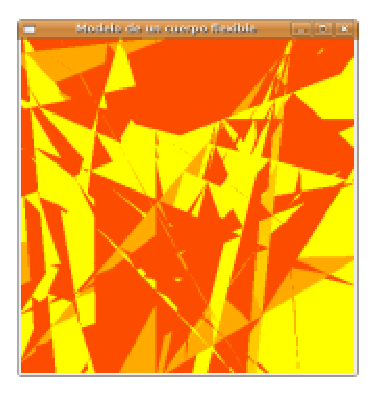
\includegraphics[]{Img/modRes4}
 \caption[Explosión por inestabilidad numérica]{La animación explota por inestabilidad numérica}
 \label{res:test4}
\end{figure}

\begin{figure}
 \centering
 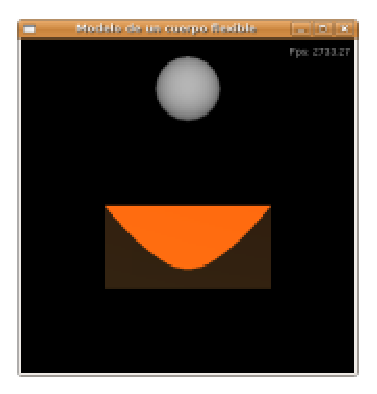
\includegraphics[]{Img/modRes5}
 \caption[Ejecución con fuerza del gas y rigidez al máximo]{El gas está al máximo $k_g=$2000.0 al igual que la rigidez de los resortes $k_s=$2.0}
 \label{res:test5}
\end{figure}

\begin{figure}
 \centering
 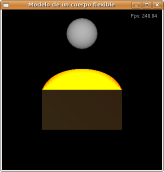
\includegraphics[]{Img/modRes6}
 \caption[Ejecución con fuerza del gas y rigidez pequeña]{El cuerpo flexible se infla como consecuencia del gas la máximo y $k_s$ pequeña}
 \label{res:test6}
\end{figure}

\section{Presentación de resultados}

Una manera de medir la eficiencia tanto de la implementación como del modelo es ver cuánto se tarda en hacer los cálculos el programa antes de pintar un frame. 
Esta medida de rendimiento es calculada comúnmente en las simulaciones gráficas y por ello me decidí a implementarla.
Como ya se dijo, esto es dependiente del hardware, así que aquí presento dos tipos de análisis.

En la primera parte, se deja como constante el hardware, hago las pruebas en la misma computadora y se varían los cálculos que se hacen en la ejecución del programa.

En la segunda parte se mantienen constantes los cálculos en el programa y se ejecuta en varios ambientes de pruebas (diferentes máquinas y distintos sistemas operativos).

\subsection{Desempeño del programa}

La medida mas comúnmente usada es el número de cuadros que la aplicación pinta en un segundo o fps (de abreviar en inglés \emph{\foreignlanguage{english}{frames per second}}).
La rutina que calcula los fps se implementó con el siguiente código dentro de la función con el registro de callback idle.

\begin{verbatim}
frame++;
time = glutGet(GLUT_ELAPSED_TIME);
if (time - timebase > 1000) {
  fps = frame * 1000.0 / (time - timebase);
  timebase = time;
  frame = 0;
}\end{verbatim}

En donde la variable global \verb|frame|, ya fue inicializada la primera vez en ceros.
Esta rutina mide los frames por segundo, que después son desplegados en la parte superior izquierda de la pantalla.

Estas pruebas fueron realizadas en la máquina ya descrita antes en la sección~\ref{maquina:trabajo}.

Las variantes consideradas son las siguientes:

\begin{description}
 \item[Estado de la animación:]la animación puede estar en pausa o en movimiento, cuando está en pausa, se pueden cambiar la opciones de render y de la rotación de la cámara, pero el programa deja de hacer los cálculos del método numérico y por ende de la acumulación de fuerzas.
 \item[Hay colisiones:]la rutina de detección de colisiones siempre es ejecutada, sin embargo sólo en caso de que se detecte una colisión se llama a la rutina de respuesta de las colisiones.
 \item[Método Numérico:]el programa ejecuta uno de dos métodos numéricos para calcular el estado siguiente de la animación, puede ser por Euler o por Runge Kutta, de donde este último requiere de casi cuatro veces mas cálculos.
 \item[Fuerza del gas:]calcular la fuerza del gas requiere de hacer cálculos sobre el área y el volumen del cuerpo flexible, cuando esta fuerza está apagada, los cálculos se omiten.
 \item[Opciones de \emph{\foreignlanguage{english}{render}}:]las opciones del \emph{\foreignlanguage{english}{render}} hacen que se tengan que hacer cálculos de la iluminación y dar color a los objetos con base a dichos cálculos.
\end{description}

La nomenclatura de la prueba usando estas variables se especifica en el cuadro~\ref{nomenclatura:prueba}.

Cada una de las variantes arriba mencionadas puede tener dos valores.
El \emph{\foreignlanguage{english}{render}} puede tener muchos valores pero para hacer las pruebas sólo voy a considerar dos: prendido, cuando se dibujan todos los cuerpos en estado sólido con iluminación y apagado, cuando se dibuja en wireframe sin luz y no se dibuja la caja del cuerpo flexible.

\begin{table}
\ra{1.2}
\begin{center}
\begin{tabular} {@{}llp{10cm}@{}}
\toprule
 Variable & Valores & Explicación\\
\midrule 
 Animación & 0 ó 1 & Se considera 1 cuando la animación esta en marcha, y 0 cuando está en pausa. \\
 Colisiones & 0 ó 1 & Se considera 1 cuando hay una colisión y se ejecuta la respuesta, 0 cuando no hay colisión y sólo se ejecuta la detección. \\
 Método Numérico & 0 ó 1 & Se considera 1 cuando se ejecuta Runge Kutta y 0 cuando se ejecuta Euler. \\
 Fuerza del gas & 0 ó 1 & Se considera 1 cuando está prendida y 0 cuando está apagada. \\
 Render & 0 ó 1 & Se considera 1 cuando se hace la mayor cantidad render, como se explicó arriba y 0 cuando se hace el mínimo posible. \\
\bottomrule
\end{tabular}
\end{center}
\caption[Explicación de la nomenclatura de la prueba del programa]{Nomenclatura de la prueba}
\label{nomenclatura:prueba}
\end{table}

Se tienen pues cinco posibles variantes, cada una con dos valores.
Se ejecutaron los 18 casos posibles (la animacion apagada implica que haya opciones que no tengan sentido, por eso son sólo 18 en vez de 32) y para cada caso anoté entre qué valores oscilan los fps. Los resultados se resumen en la tabla~\ref{resultado:prueba1}.

La razon por la cual los fps, son un rango es que al momento de la ejecución, cada segundo varía el valor de los fps.
Es por eso que al hacer el experimento con las condiciones de cada caso, anote tanto el valor máximo que alcanzaron lo fps, como el valor mínimo; esto es lo que llamo el rango.

La columna de contribución, representa cuánto contribuye a los cálculos la prueba en cuestión con respecto a que se hacen \emph{todos} los cálculos, tomando como base el caso en que todas las variables están prendidas.
La contribución $C$ es calculada de la siguiente manera:

$$ C = \frac{FPS_{min} + FPS_{max}}{2} \div FPS_{base}$$

En donde $FPS_{min}$ es el mínimo de fps en cada categoría y $FPS_{max}$ es el máximo de fps en la misma, $FPS_{base}$ es el promedio de fps de la categoría base, para este caso $FPS_{base} =$ 210.81 dado que es el promedio de los $FPS$ de la prueba que más poder requiere y se presenta en el último renglón de la tabla.

\begin{table}
\ra{1.2}
\begin{center}
%\begin{tabular} {|c|c|c|c|c|c|c|}
\begin{tabular} {@{}cccccrr@{}}
\toprule
 Anim & Coli & Método & F. Gas & Render & FPS & Contr\\
\midrule
 0 & n/a & n/a & n/a & 0 & 2753.08 - 2768.15 & 0.08\\
 0 & n/a & n/a & n/a & 1 & 2754.01 - 2826.18 & 0.08\\
 1 & 0 & 0 & 0 & 0 & 654.35 - 663.34 & 0.32\\
 1 & 0 & 0 & 0 & 1 & 620.38 - 630.37 & 0.34\\
 1 & 0 & 0 & 1 & 0 & 501.04 - 512.98 & 0.42\\
 1 & 0 & 0 & 1 & 1 & 464.03 - 491.02 & 0.44\\
 1 & 0 & 1 & 0 & 0 & 447.99 - 456.54 & 0.47\\
 1 & 0 & 1 & 0 & 1 & 454.09 - 474.05 & 0.45\\
 1 & 0 & 1 & 1 & 0 & 240.52 - 251.99 & 0.86\\
 1 & 0 & 1 & 1 & 1 & 203.57 - 212.57 & 1.01\\
 1 & 1 & 0 & 0 & 0 & 640.72 - 660.54 & 0.32\\
 1 & 1 & 0 & 0 & 1 & 612.76 - 627.74 & 0.34\\
 1 & 1 & 0 & 1 & 0 & 499.03 - 512.03 & 0.42\\
 1 & 1 & 0 & 1 & 1 & 470.06 - 484.52 & 0.44\\
 1 & 1 & 1 & 0 & 0 & 347.31 - 357.29 & 0.60\\
 1 & 1 & 1 & 0 & 1 & 333.67 - 342.32 & 0.62\\
 1 & 1 & 1 & 1 & 0 & 214.34 - 219.26 & 0.97\\
 1 & 1 & 1 & 1 & 1 & 209.04 - 212.57 & 1.00\\
\bottomrule
\end{tabular}
\end{center}
\caption[Resultados de la prueba del programa]{Resultados primera prueba}
\label{resultado:prueba1}
\end{table}

Hay algunos datos interesantes con respecto a la tabla \ref{resultado:prueba1}, por ejemplo el hecho de lo poco que contribuye el render al desempeño de la animación (el .03).
Esto se explica por que cuando el render está apagado se trazan más objetos gráficos, se dibujan cuatro lineas y cuatro puntos por cada cara, mientras que cuando el render está prendido si bien se hacen cálculos de iluminación sólo se dibuja un cuadro por cada cara.

También de la tabla, puedo concluir  que lo que más contribuye al desempeño de la animación es el método numérico usado, pues como dijimos el
método de RK4, lleva casi cuatro veces más cálculos que el método de Euler (en la tabla se ve que representa el .56 de los cálculos).

El otro factor que hace considerablemente más lenta la animación es el cálculo de la fuerza del gas con el .48 del tiempo.

\subsection{Desempeño del programa en diferentes ambientes}

La última prueba consistió en hacer constante la ejecución del programa y ver qué desempeño tiene en diferentes tipos de hardware.

Para esta  prueba se ejecutó el programa en diferentes ambientes.
En cada ambiente se consideran importantes sólo las siguientes características: la memoria principal, el sistema operativo, el procesador, la arquitectura y si hay o no memoria de vídeo.

La ejecución del programa se hizo de una manera típica, lo que haciendo una equivalencia con la prueba anterior es que esté en marcha la animación, que haya colisiones con el método de Runge Kutta, que haya fuerza del gas y que el \emph{\foreignlanguage{english}{render}} se haga completo.
También se hizo la ejecución con las siguientes características mínimas: método de Euler y sin fuerza de gas.
De ambas pruebas se miden los fps.

Los resultados se listan a continuación.
\begin{itemize}
 \item Sistema Operativo: Ubuntu 7.04
 \item Procesador: Opteron 1214 a 2.2GHz
 \item Memoria RAM: 2.0GB
 \item Memoria de Video: Tarjeta Nvidia FX3500, 256MB, driver propietario
 \item Velocidad en prueba mínima: 612.76 - 627.74fps
 \item Velocidad en prueba normal: 209.04 - 212.57fps
\end{itemize}

\begin{itemize}
 \item Sistema Operativo: Windows XP professional edition
 \item Procesador: AMD Duron a 1.2GHz
 \item Memoria RAM: 512MB
 \item Memoria de Video: Tarjeta Nvidia 64MB
 \item Velocidad en prueba mínima: 72.0 - 102.0fps
 \item Velocidad en prueba normal: 60.0 - 94.0fps
\end{itemize}

La última prueba se llevó a cabo en una máquina virtual, con el fin de evaluar los requerimientos mínimos.

\begin{itemize}
 \item Sistema Operativo: Windows XP professional edition
 \item Procesador: Dual Core AMD Opteron 999Mhz
 \item Memoria RAM: 256MB
 \item Memoria de Video: Ninguna, adaptador VM-Ware SVG 2
 \item Velocidad en prueba mínima: 65.40 - 71.72fps
 \item Velocidad en prueba normal: 46.44 - 52.22 fps
\end{itemize}

